% =====================================================================
% APPENDICES
% =====================================================================

\chapter{Tracker SMS Configuration Commands}
\label{app:sms}
The Concox GT06S tracker is configured entirely over SMS; each command
is acknowledged by a return SMS from the device. Table~\ref{tab:sms}
lists the commands used during deployment and the pilot.

\begin{table}[H]
\caption{GT06S SMS commands used in this work.}
\label{tab:sms}
\centering
\small
\begin{tabular}{@{}lp{9.6cm}@{}}
\toprule
\textbf{Command} & \textbf{Effect} \\
\midrule
\texttt{TIMER,5,300\#} & Set asymmetric reporting: every 5\,s while the
vehicle is moving, every 300\,s while static. This is the device-side
half of the idle-efficiency optimization
(Section~\ref{sec:eval-efficiency}). \\
\texttt{PARAM\#} & Read back the active configuration, used to verify
that the \texttt{TIMER} change was applied. \\
\texttt{STATUS\#} & Report battery level and GSM/GPS state, used for
routine health checks during the pilot. \\
\bottomrule
\end{tabular}
\end{table}

The device also emits a low-frequency heartbeat between position
reports, which keeps it visible as \emph{online} to the telematics
server while parked.

\chapter{Operator-Configurable Processing Parameters}
\label{app:params}
Table~\ref{tab:params} consolidates the tunable parameters of the
position-processing pipeline with the values used in the pilot. All are
operator-configurable without code changes.

\begin{table}[H]
\caption{Pipeline parameters and pilot values.}
\label{tab:params}
\centering
\small
\begin{tabular}{@{}lll@{}}
\toprule
\textbf{Parameter} & \textbf{Pilot value} & \textbf{Role} \\
\midrule
Accuracy soft-reject      & 120\,m      & Quality gate
(Section~\ref{sec:design-filter}) \\
Accuracy hard-reject      & 250\,m      & Quality gate \\
Teleport guard            & 120\,km/h   & Physical plausibility \\
Minimum movement          & 4\,m        & Stationary-jitter floor \\
Reliable-speed threshold  & 5\,km/h     & ETA effective speed
(Section~\ref{sec:design-eta}) \\
Default speed             & 20\,km/h    & ETA fallback speed \\
Arrival radius            & 80\,m       & Stop-reached detection, alerts \\
Staleness check period    & 30\,s       & Trip staleness job \\
Active-trip poll interval & 8\,s        & Traccar reconciliation \\
Idle poll interval        & 60\,s       & Trip-aware throttling \\
Moving report interval    & 5\,s        & Device cadence (GT06S) \\
Parked report interval    & 300\,s      & Device cadence (GT06S) \\
\bottomrule
\end{tabular}
\end{table}

\chapter{API Surface: Functional Overview}
\label{app:api}
The application server exposes one REST API consumed by both clients,
plus the Socket.IO realtime gateway. Table~\ref{tab:api} summarizes the
API at the level of functional resource areas, indicating which client
consumes each area. (Exact endpoint paths are an implementation detail
and are omitted here; the table records the functional surface.)

\begin{table}[H]
\caption{Functional overview of the API surface.}
\label{tab:api}
\centering
\small
\begin{tabular}{@{}lp{6.6cm}l@{}}
\toprule
\textbf{Resource area} & \textbf{Operations} & \textbf{Consumer} \\
\midrule
Authentication & Registration, login, session management, OTP
verification & Both clients \\
Routes \& stops & Query route geometry, stop lists; create and edit
routes (route builder) & Both / Admin \\
Schedules & Query today's and upcoming schedules; manage timetable
entries & Both / Admin \\
Trips \& live state & Query active trip, live tracking state, and
per-stop ETAs & Passenger \\
Driver location & Publish authenticated fallback position reports &
Driver mode \\
Favourites \& alerts & Manage favourite stops and drop-off alert
subscriptions & Passenger \\
Notifications & Deliver and mark-read arrival/service notifications &
Passenger \\
Fleet \& devices & Manage buses, GPS devices, and driver assignments &
Admin \\
Users \& roles & Manage accounts and role-based permissions & Admin \\
Realtime (Socket.IO) & Join per-trip rooms; receive position and ETA
push events & Passenger / Admin \\
\bottomrule
\end{tabular}
\end{table}

\chapter{Passenger Application Screens}
\label{app:screens}
This appendix reproduces screens of the deployed passenger application,
captured on an Android device during operation on the real routes.
Figure~\ref{fig:screens-app} shows the core tracking experience;
Figure~\ref{fig:screens-alerts} shows the alerting and engagement
surfaces, including the honest edge-condition states discussed in
Section~\ref{sec:impl-passenger}.

\begin{figure}[H]
\centering
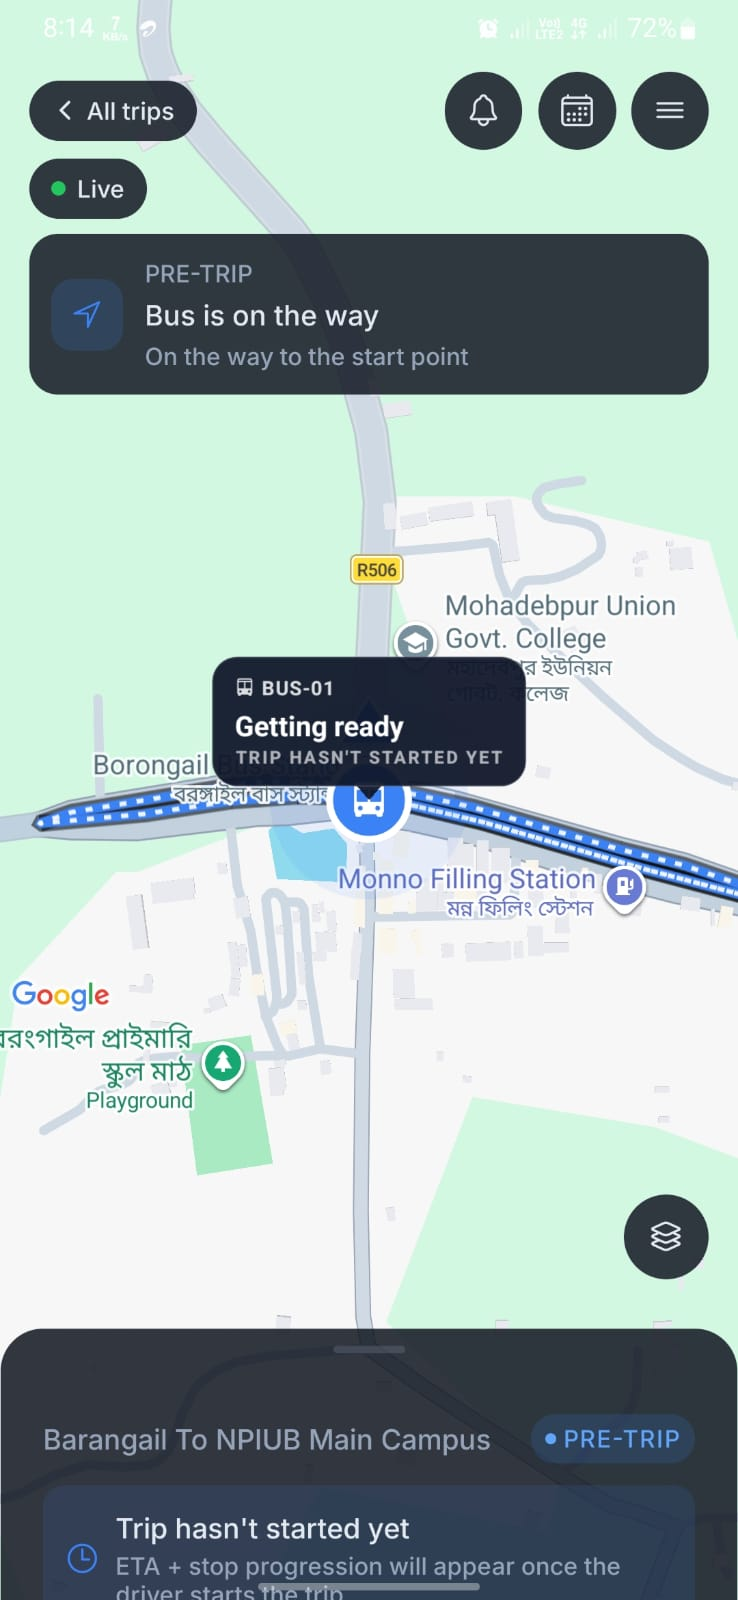
\includegraphics[width=0.235\textwidth]{shots/pretrip_map.jpg}\hfill
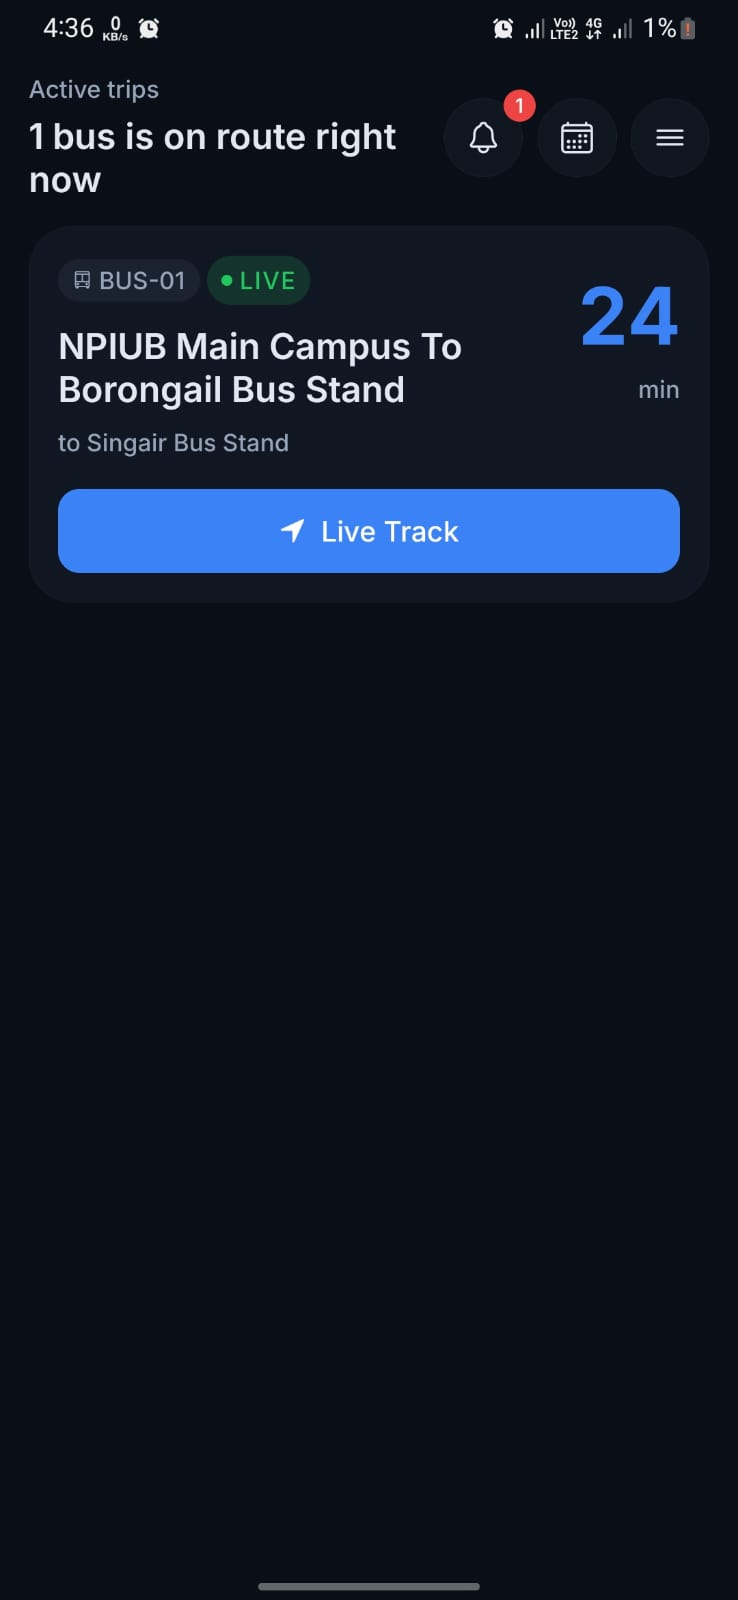
\includegraphics[width=0.235\textwidth]{shots/active_trip.jpg}\hfill

\includegraphics[width=0.235\textwidth]{shots/schedules.jpg}\hfill
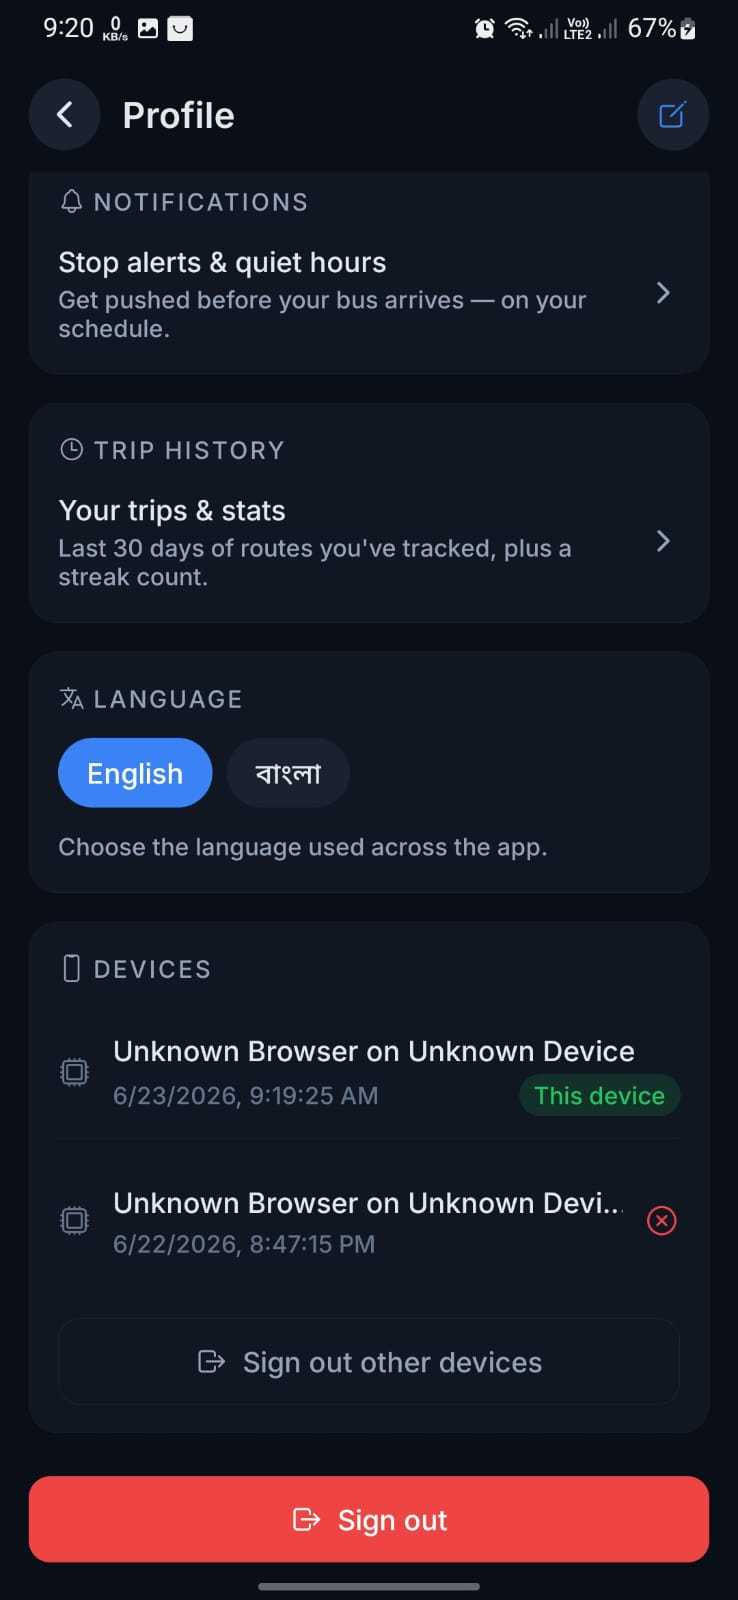
\includegraphics[width=0.235\textwidth]{shots/language.jpg}
\caption[Core tracking screens of the passenger application]{Core
tracking experience. Left to right: (a) the live map during the
\textsc{pre\_trip} window---the bus is rendered at its pre-departure
position with a ``getting ready'' state, so the map is never blank
before departure; (b) the active-trips view showing a live bus
(\textsc{bus-01}) on route with its ETA to the rider's stop and a
one-tap \emph{Live Track} action; (c) today's schedules grouped by day
and route; (d) the in-app language setting with the English/Bangla
toggle.}
\label{fig:screens-app}
\end{figure}

\begin{figure}[H]
\centering
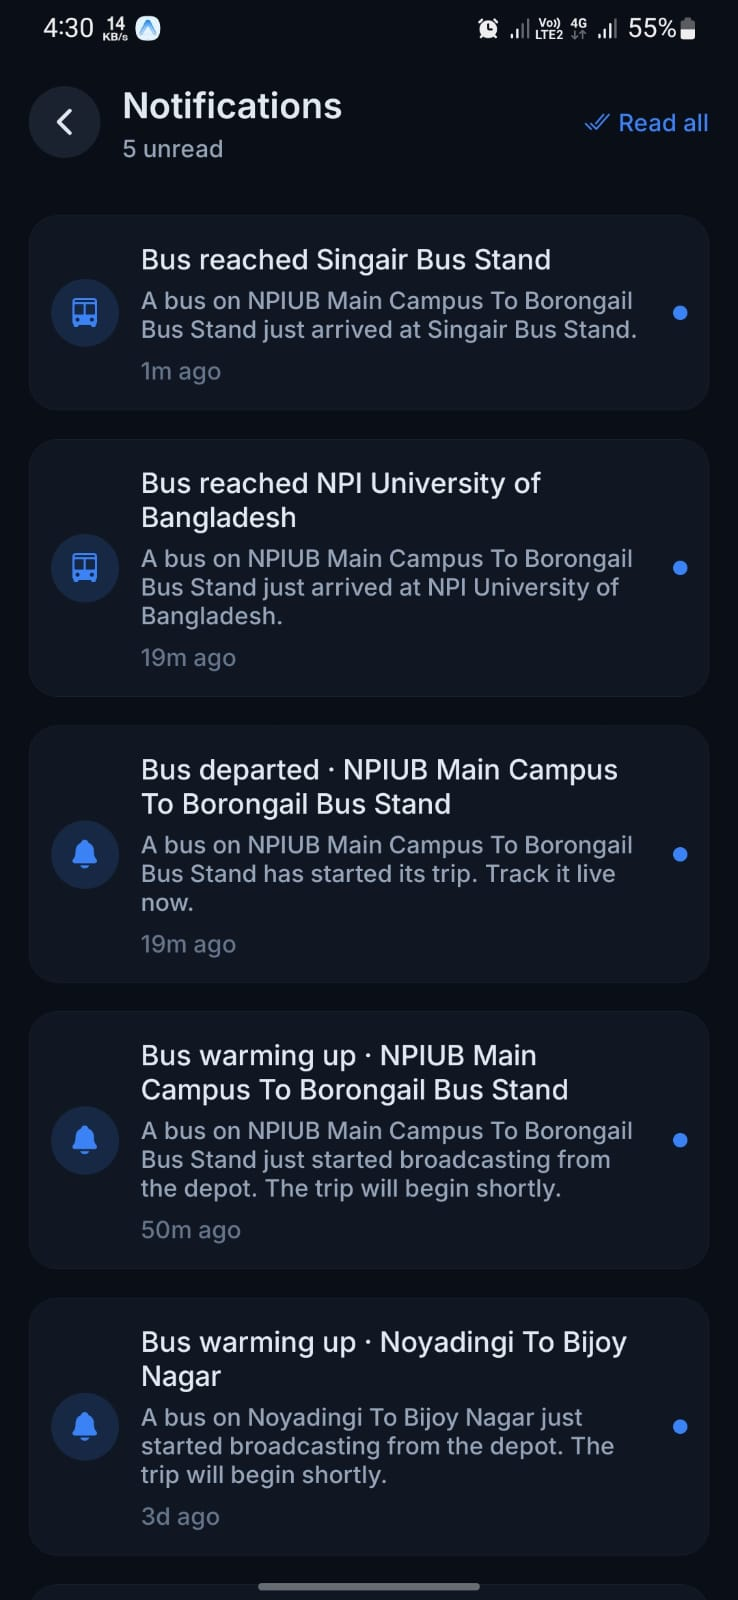
\includegraphics[width=0.235\textwidth]{shots/notif_list.jpg}\hfill
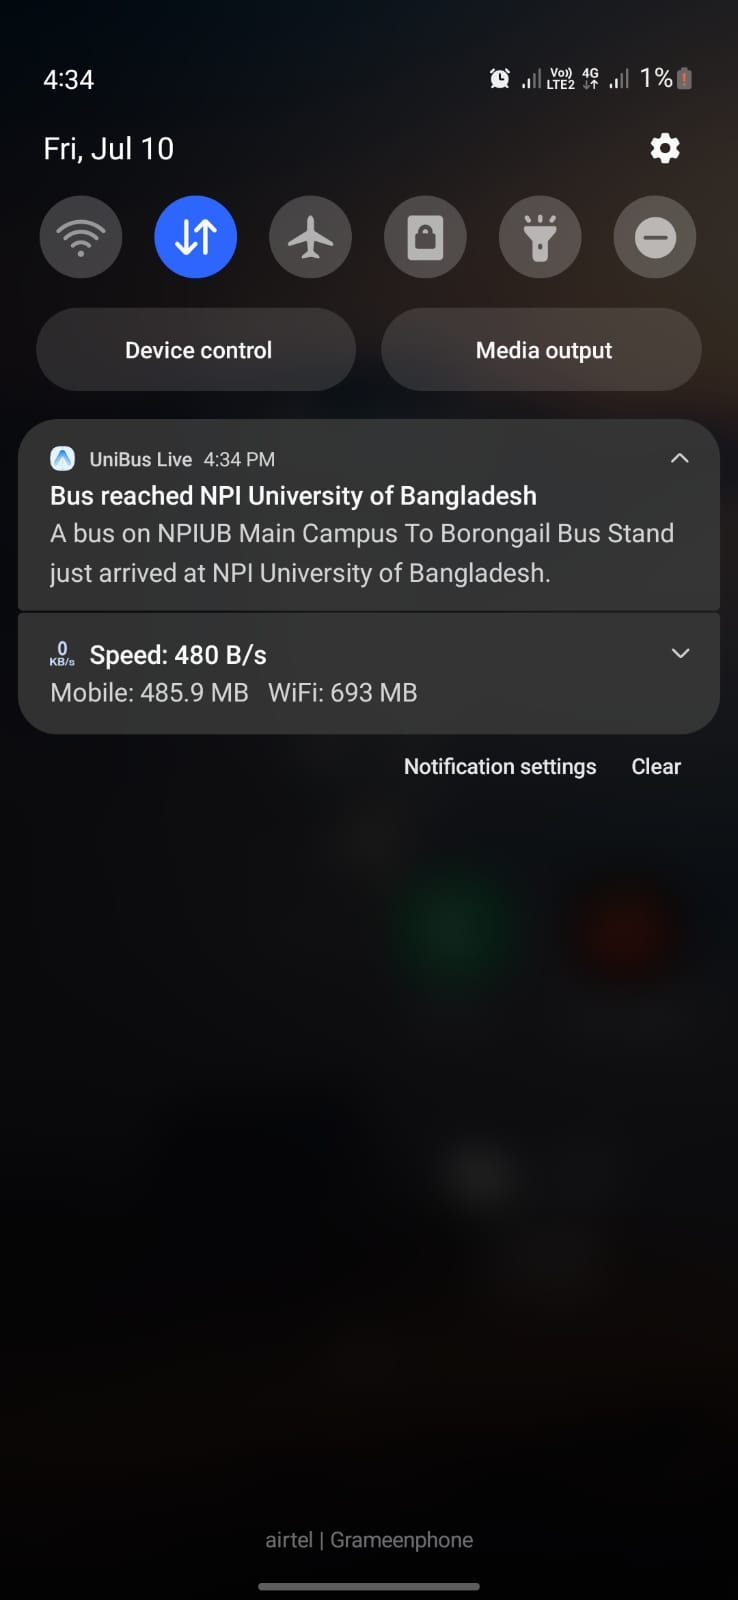
\includegraphics[width=0.235\textwidth]{shots/notif_shade.jpg}\hfill
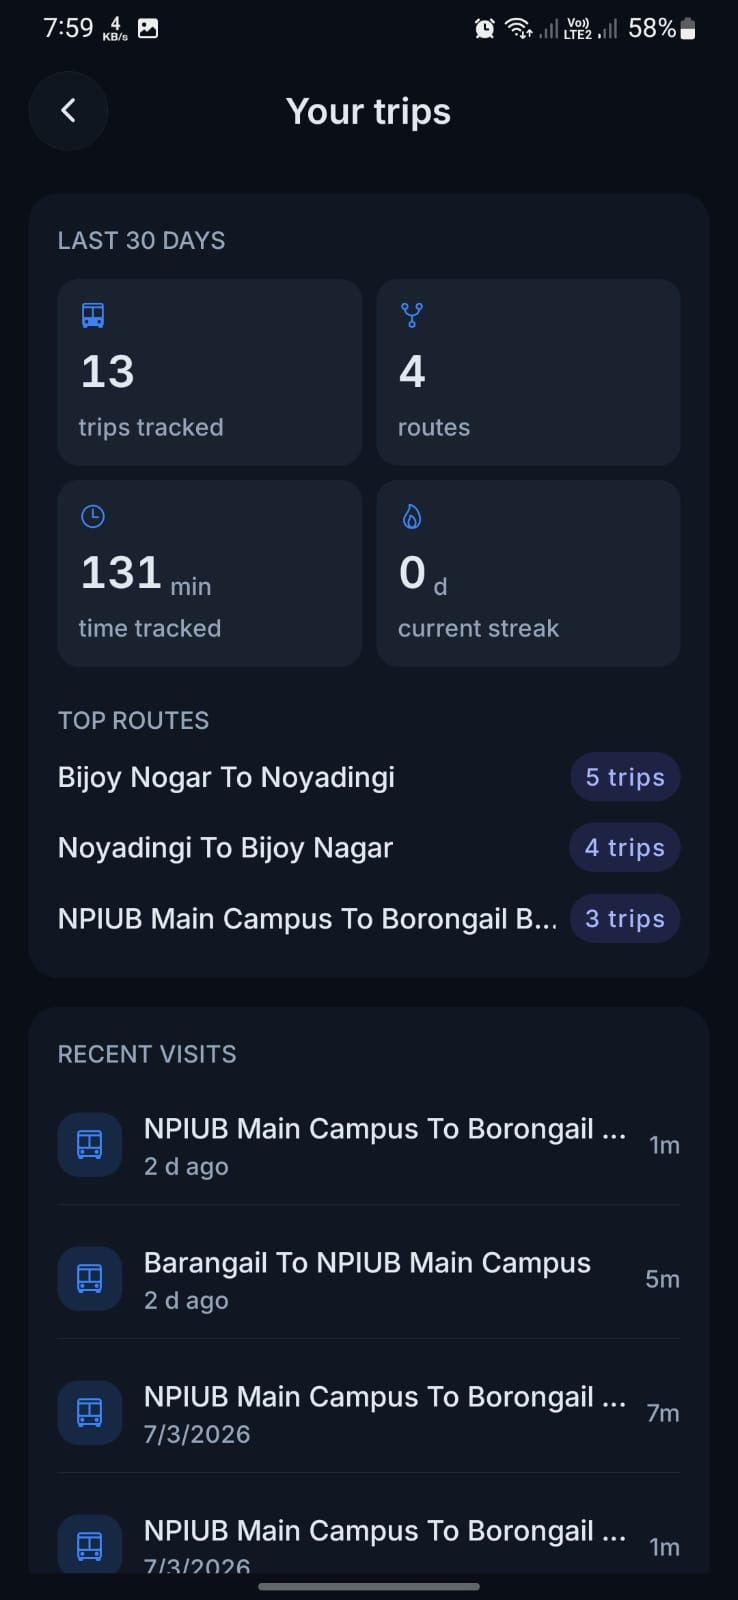
\includegraphics[width=0.235\textwidth]{shots/trip_stats.jpg}\hfill
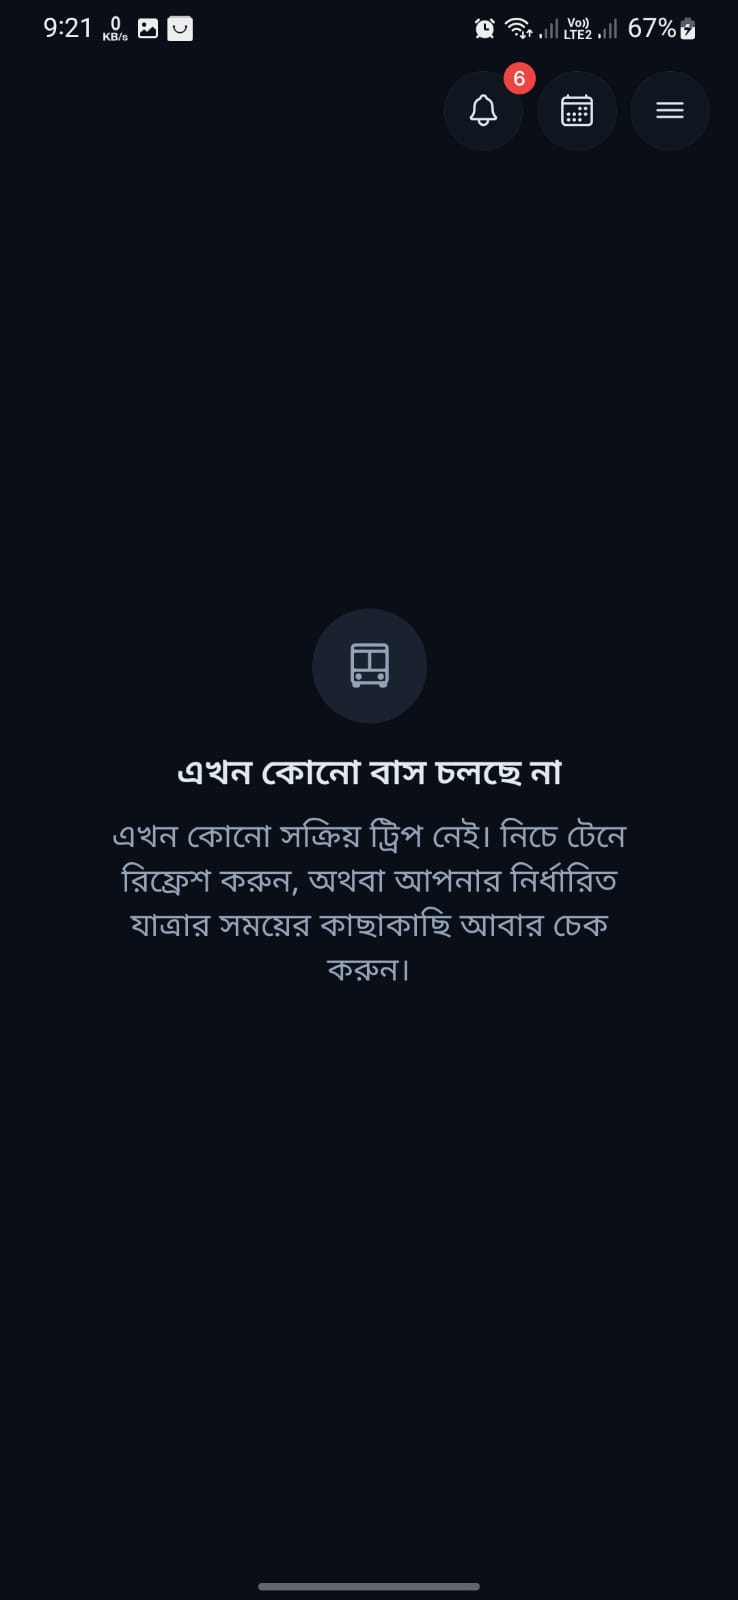
\includegraphics[width=0.235\textwidth]{shots/empty_bn.jpg}
\caption[Alerting and engagement screens]{Alerting and engagement
surfaces. Left to right: (a) the in-app notification feed recording trip
events (bus warming up, departed, reached a stop); (b) a system push
notification delivered outside the app announcing that the bus reached
the campus; (c) the rider's trip history and statistics (trips tracked,
routes used, time tracked); (d) the Bangla-localized empty state shown
when no bus is currently running---an example of the fully bilingual
interface (FR-10).}
\label{fig:screens-alerts}
\end{figure}

\chapter{Administration Console Screens}
\label{app:adminscreens}
This appendix reproduces the management pages of the web administration
console that complement the principal screens shown in
Figure~\ref{fig:admin}. All screens were captured from the deployed
console operating on the real fleet data.

\begin{figure}[H]
\centering
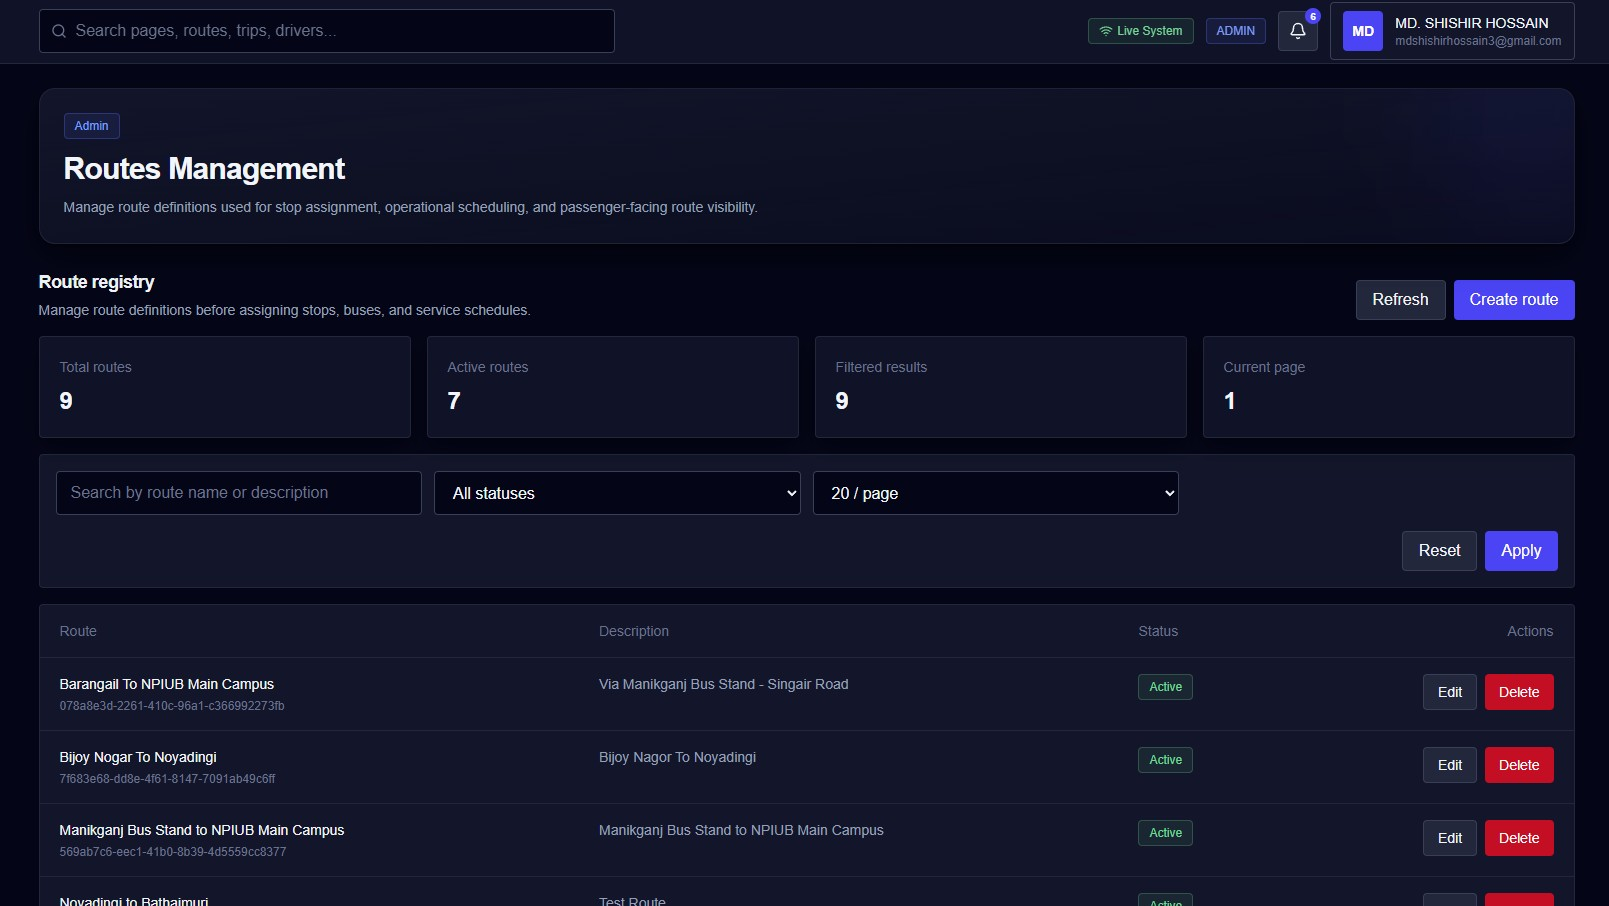
\includegraphics[width=0.49\textwidth]{admin/routes.jpg}\hfill
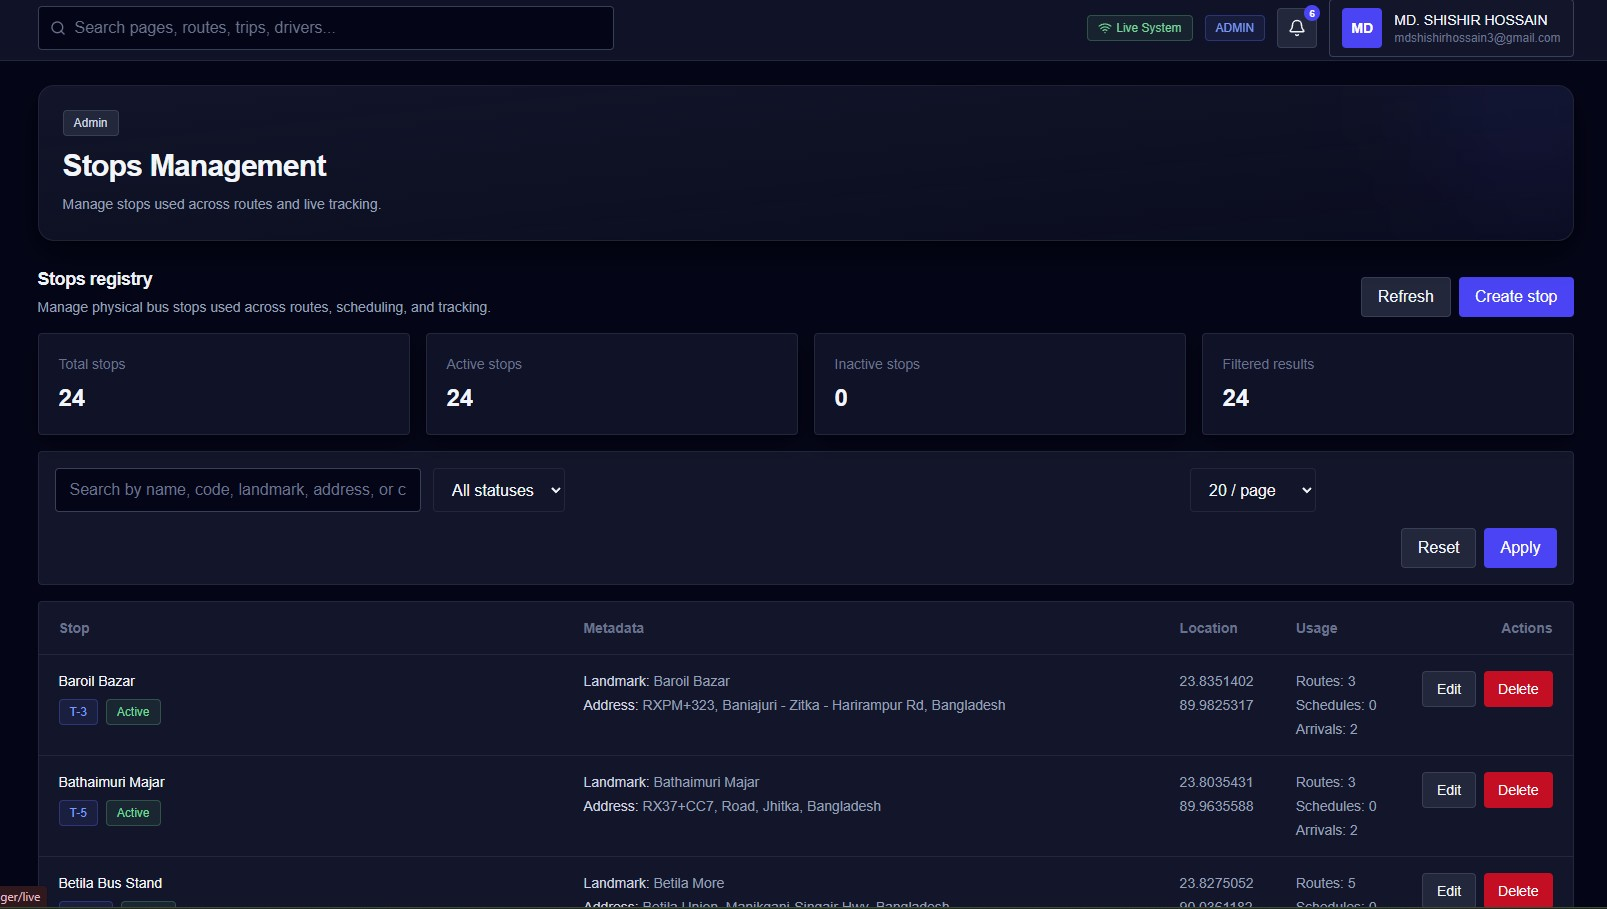
\includegraphics[width=0.49\textwidth]{admin/stops.jpg}\\[2mm]
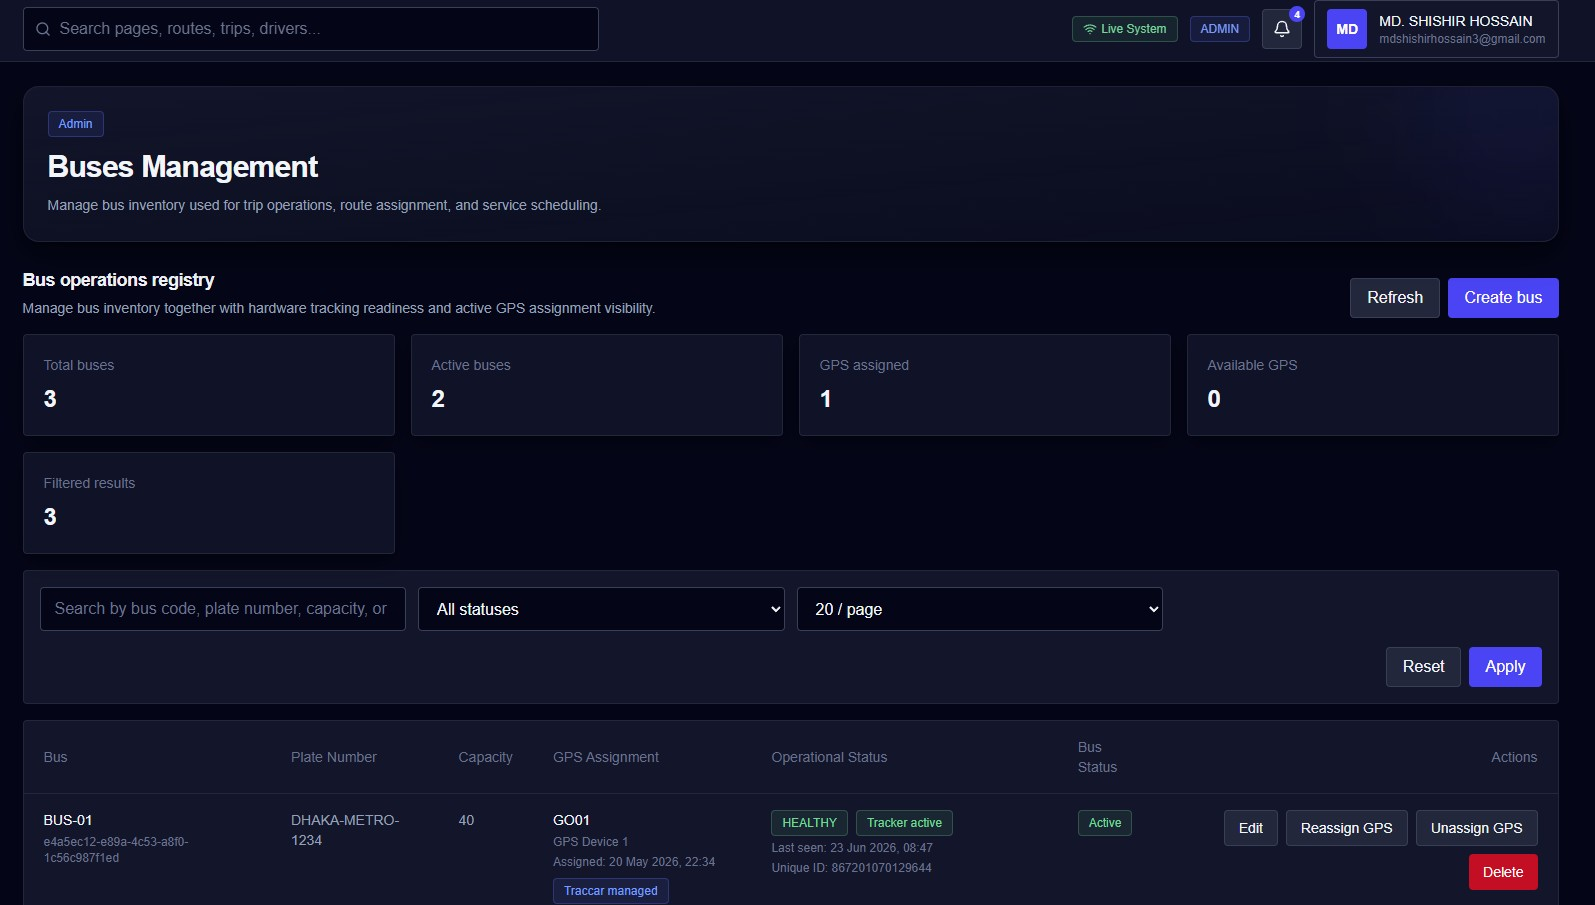
\includegraphics[width=0.49\textwidth]{admin/buses.jpg}\hfill
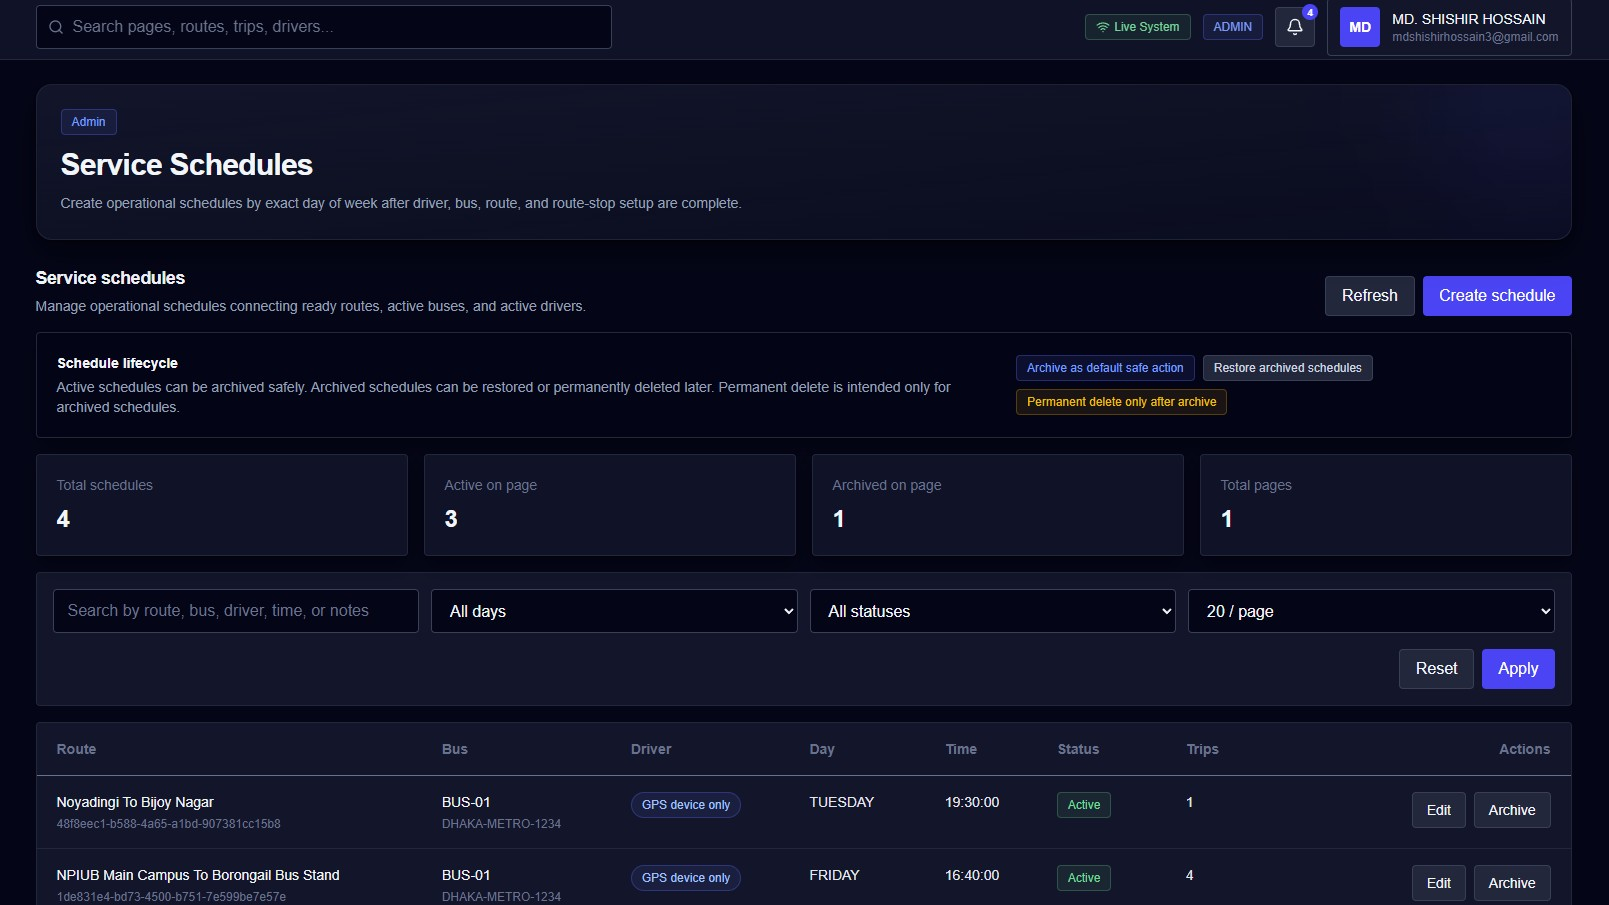
\includegraphics[width=0.49\textwidth]{admin/schedules.jpg}
\caption[Management pages of the administration console]{Management
pages of the administration console. Top left: the route registry with
per-route status and stop-visibility settings. Top right: stops
management, maintaining the physical bus stops used across routes.
Bottom left: bus operations registry, pairing each bus with its hardware
tracking readiness and GPS assignment. Bottom right: service schedules,
binding routes, buses, drivers, days, and departure times.}
\label{fig:admin-mgmt}
\end{figure}

\begin{figure}[H]
\centering
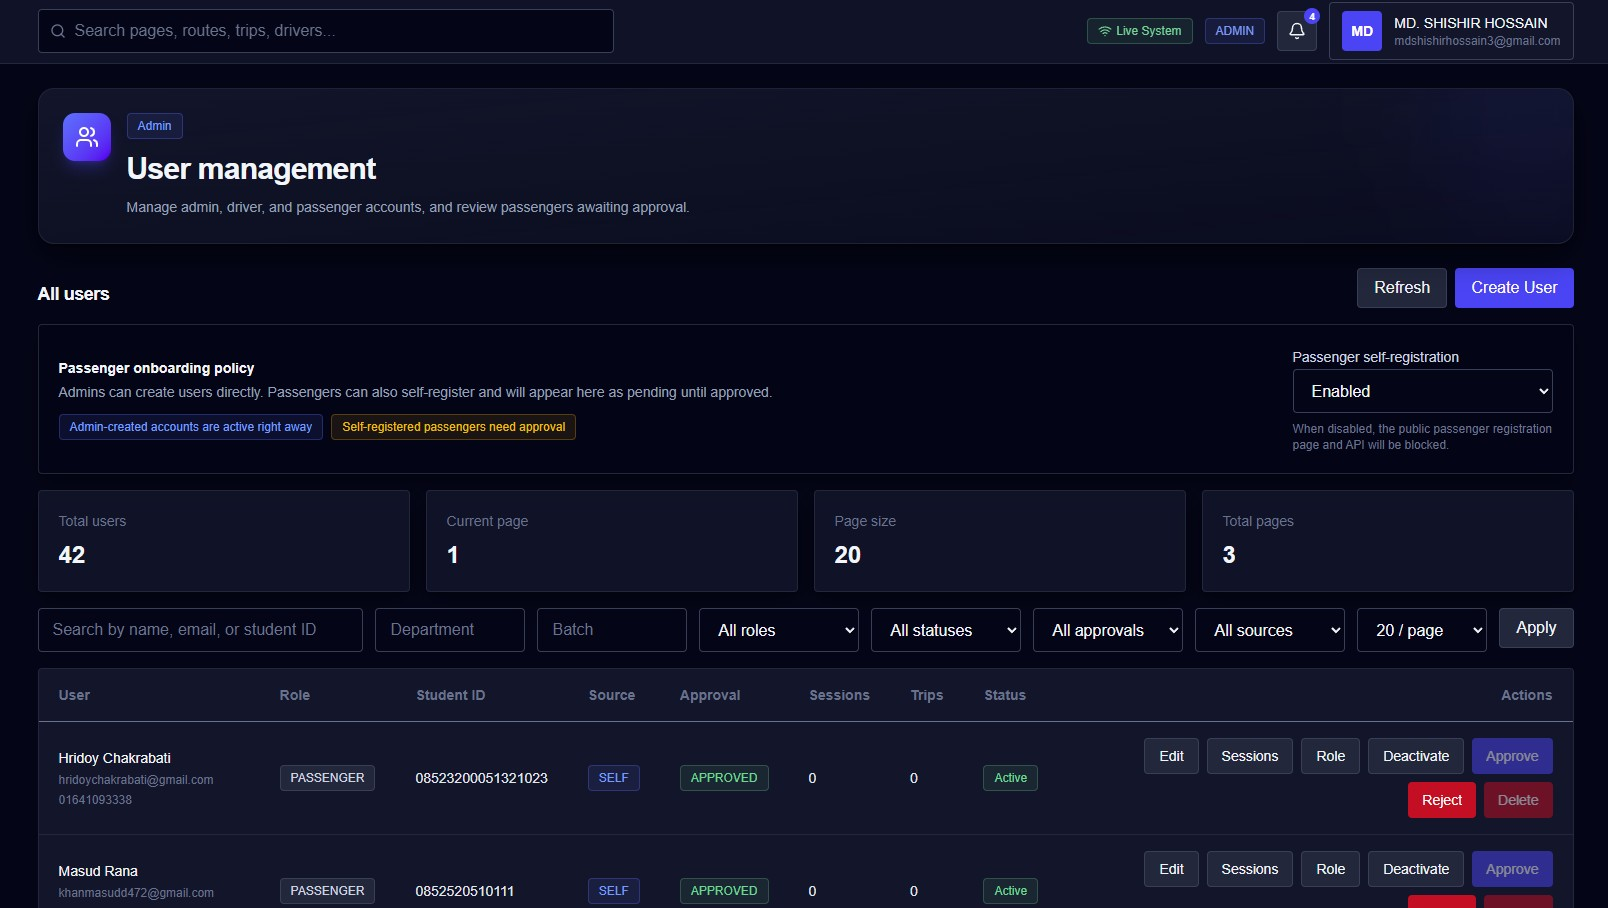
\includegraphics[width=0.85\textwidth]{admin/users.jpg}
\caption[User management page]{The user management page: accounts,
roles, per-user sessions, and the passenger onboarding approval policy
(NFR-5).}
\label{fig:admin-users}
\end{figure}
